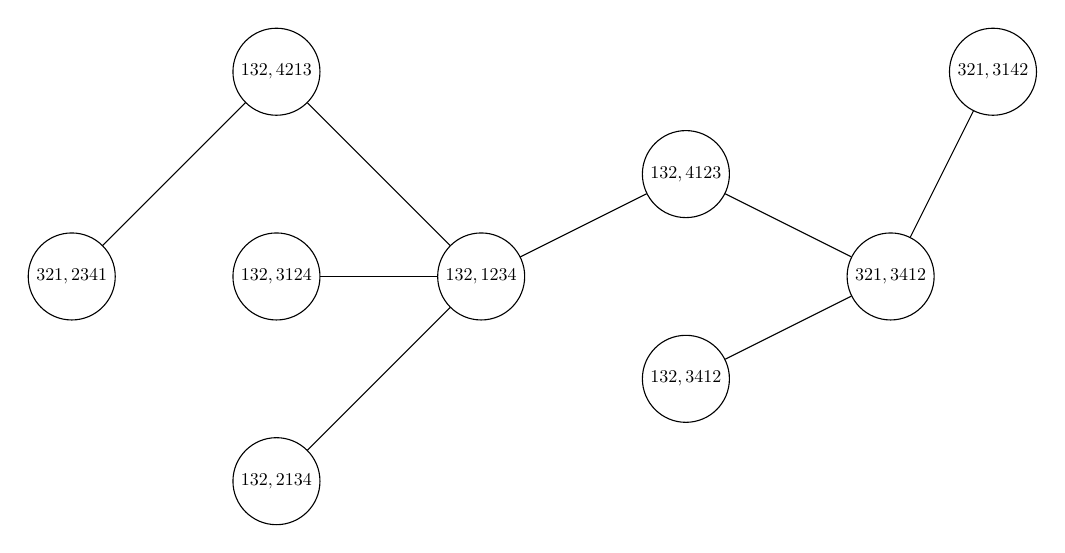
\begin{tikzpicture}[vertex/.style = {shape=circle,draw,minimum size=1.5em},scale=0.65, every node/.style={scale=0.65}]
    \node[vertex] (a) at (-12,0) {$\Av{321, 2341}$};%0-a
    \node[vertex] (b) at (4,0) {$\Av{321, 3412}$};%1-b
    \node[vertex] (c) at (6,4) {$\Av{321, 3142}$};%2-c
    \node[vertex] (d) at (-4,0) {$\Av{132, 1234}$};%3-d
    \node[vertex] (e) at (-8,4) {$\Av{132, 4213}$};%4-e
    \node[vertex] (f) at (0,2) {$\Av{132, 4123}$};%5-f
    \node[vertex] (g) at (-8,0) {$\Av{132, 3124}$};%6-g
    \node[vertex] (h) at (-8,-4) {$\Av{132, 2134}$};%7-h
    \node[vertex] (i) at (0,-2) {$\Av{132, 3412}$};%8-i
    \draw (a) -- (e);
    \draw (d) -- (e);
    \draw (d) -- (f);
    \draw (d) -- (g);
    \draw (d) -- (h);
    \draw (b) -- (f);
    \draw (b) -- (c);
    \draw (b) -- (i);
\end{tikzpicture}